\chapter{Distribuciones continuas más usuales}

\section{Distribución Uniforme}

\begin{defi}
Se dice que una variable aleatoria $X \sim U[a,b]$ si su función de densidad es 
\begin{align*}
    f_X(x) = \left\{ \begin{array}{lcc}
             \frac{1}{b - a} &  si  & a \leq x \leq b\\
             0 &  si  & resto\\
             \end{array}
        \right. .
\end{align*}
\end{defi}

\begin{obs}
Si $X \sim U[a,b]$ entonces
\begin{itemize}
    \item Su función de distribución es
    \begin{align*}
        F_X(x) = \left\{ \begin{array}{lcc}
             0 &  si  & x < a\\
             \frac{x - a}{b - a} &  si  & a \leq x < b\\
             1 &  si  & x \ge b\\
             \end{array}
        \right. .
    \end{align*}
    \item $P(x \leq X \leq x + \Delta x) = \frac{\Delta x}{b - a}$.
    \item $E[X] = \frac{b + a}{2}$.
    \item $V[X] = \frac{(b -a)^2}{12}$.
    \item $M_X(t) = E[e^{tx}] = \int_{a}^{b}{e^{tx}\frac{1}{b -a } \ dx} = \frac{e^{tb} - e^{ta}}{t(b -a )}$, si $t \not = 0$. Entonces
    \begin{align*}
        M_X(t) = \left\{ \begin{array}{lcc}
             \frac{e^{tb} - e^{ta}}{t(b -a )} &  si  & t \not = 0\\
             0 &  si  & t = 0\\
             \end{array}
        \right. .
    \end{align*}
\end{itemize}
\end{obs}

\begin{prop}
Sea X una variable aleatoria y $F_X$ su función de distribución con $F_X$ estrictamente creciente. Entonces $Y = F(X)$ es una variable aleatoria e $Y \sim U(0,1)$.
\end{prop}

\begin{proof}
El soporte de $Y$ es $S_Y = [0,1]$.
\begin{itemize}
    \item Si $y < 0$, es claro que $F_Y(y) = 0$.
    \item Si $0 \leq y < 1$
    \begin{align*}
        F_Y(y) = P(Y \leq y) = P(F(x) \leq y) = P(X \leq F^{-1}(y)) = F(F^{-1}(y)) = y.
    \end{align*}
    \item Si $y \ge 1$, es claro que $F_Y(y) = 1$.
\end{itemize}
Por tanto
\begin{align*}
    F_Y(y) = \left\{ \begin{array}{lcc}
             0 &  si  & x < 0\\
             y &  si  & 0 \leq x < 1\\
             1 &  si  & x \ge 1\\
             \end{array}
        \right. .
\end{align*}
lo que nos dice que $Y \sim U(0,1)$.
\end{proof}

\section{Distribución Normal}

\begin{defi}
Se dice que una variable aleatoria $X \sim N(\mu, \sigma)$, $\mu \in \mathb{R}$, $\sigma > 0$, si su función de densidad es
\begin{align*}
    f(x) = \frac{1}{\sigma \sqrt{2\pi}}e^{-\frac{1}{2}\frac{(x - \mu)^2}{\sigma^2}}, \ x \in \mathbb{R}.
\end{align*}
\end{defi}

\begin{obs}
Si $X \sim N(\mu, \sigma)$ entonces
\begin{itemize}
    \item $E[X] = \mu$.
    \item $D(X) = \sigma$.
    \item Si $Z \sim N(0,1)$ entonces $E[Z] = 0$, $V[Z] = 1$ y $D(Z) = 1$.
    \item $Z = \frac{X - \mu}{\sigma}$ es variable aleatoria y $Z \sim N(0,1)$.
    \item Si $Z \sim N(0,1)$ entonces su función de densidad es
    \begin{align*}
        \phi(z) = \frac{1}{\sqrt{2\pi}}e^{-z^2/2}, \ z \in \mathbb{R}.
    \end{align*}
    Su función generatriz de momentos es
    \begin{align*}
        M_Z(t) = E[e^{tz}] = \int_{-\infty}^{+\infty}{e^{tz}\frac{1}{\sqrt{2\pi}}e^{-z^2/2} \ dz} = e^{t^2/2}
    \end{align*}
    para todo $t \in \mathbb{R}$ (para poder calcular esta integral, es útil saber que $\int_{-\infty}^{+\infty}{\frac{1}{\sqrt{2\pi}}e^{-z^2/2} \ dz} = 1$).
    \item Haciendo uso de la función generatriz de momentos de $Z \sim N(0,1)$, calculemos la función generatriz de momentos de $X \sim N(\mu, \sigma)$. La funcuión de densidad de $X$ es
    \begin{align*}
    f(x) = \frac{1}{\sigma \sqrt{2\pi}}e^{-\frac{1}{2}\frac{(x - \mu)^2}{\sigma^2}}, \ x \in \mathbb{R}.
\end{align*}
Nótese que, $Z = \frac{X - \mu}{\sigma} \sim N(0,1)$, despenjando, $X = \sigma Z + \mu$. Calculemos la función generatriz de momentos de $X$
\begin{align*}
    M_X(t) &= E[e^{tx}] = E[e^{t(\sigma z + \mu)}] = E[e^{t\sigma z} \cdot e^{t \mu}] = e^{t \mu} E[e^{(t\sigma) z}]\\
    &= e^{t \mu}M_Z(t \sigma)
\end{align*}
donde $Z \sim N(0,1)$, luego
\begin{align*}
    M_X(t) = e^{t \mu}M_Z(t \sigma) = e^{t \mu}e^{\frac{1}{2}t^2 \sigma ^2}
\end{align*}
para todo $t \in \mathbb{R}$.
\end{itemize}
\end{obs}

\begin{obs}
Si $X$ e $Y$ son varibles aleatorias independientes
\begin{enumerate}
    \item[(1)] $E[X \cdot Y] = E[X] \cdot E[Y]$.
    \item[(2)] $G_{X + Y}(s) = G_X(s) \cdot G_Y(s)$ y $M_{X + Y}(t) = M_X(t) \cdot M_Y(t)$.
    \item[(3)] $V[X + Y] = V[X] + V[Y]$ y $V[X - Y] = V[X] + V[Y]$.
\end{enumerate}
\end{obs}

\begin{prop}
\begin{enumerate}
    \item[(1)] Si $X_1, ..., X_n$ son variables aleatorias independientes tales que $X_i \sim N(\mu_i, \sigma_i)$, entonces
    \begin{align*}
        S = \sum_{i=1}^{n}{X_i} \sim N\left(\sum_{i=1}^{n}{\mu_i}, \sqrt{\sum_{i=1}^{n}{\sigma_i^2}}\right).
    \end{align*}
    \item[(2)] Si $X_1, ..., X_n$ son variables aleatorias independientes tales que $X_i \sim N(\mu, \sigma)$, entonces
    \begin{align*}
        \overline{X} = \frac{\sum_{i=1}^{n}{X_i}}{n} \sim N\left( \mu, \frac{\sigma}{\sqrt{n}}\right).
    \end{align*} 
\end{enumerate}
$\overline{X}$ se conoce como media muestral.
\end{prop}

\section{Distribución Exponencial}

\begin{defi}
Se dice que una variable aleatoria $X \sim Exp(\lambda)$, $\lambda > 0$, si su función de densidad es
\begin{align*}
    f(x) = \left\{ \begin{array}{lcc}
             0 &  si  & x < 0\\
             \lamda e^{-\lambda x} &  si  & x \ge 0\\
             \end{array}
        \right. . 
\end{align*}
\end{defi}

\begin{obs}
Si $X \sim Exp(\lambda)$ entonces
\begin{itemize}
    \item Su función de distribución es
    \begin{align*}
        F(x) = \left\{ \begin{array}{lcc}
             0 &  si  & x \leq 0\\
            1 - \lamda e^{-\lambda x} &  si  & x > 0\\
             \end{array}
        \right. . 
    \end{align*}
    \item $E[X] = \frac{1}{\lambda}$.
    \item $V[X] = \frac{1}{\lambda^2}$.
    \item $Me = \frac{\log(2)}{\lambda}$.
    \item Su función generatriz de momentos es
    \begin{align*}
        M_X(t) = \left\{ \begin{array}{lcc}
             \left( 1 - \frac{t}{\lambda} \right)^2 &  si  & t < \lambda\\
             \text{no existe} &  si  & t \ge \lambda\\
             \end{array}
        \right. . 
    \end{align*}
\end{itemize}
\end{obs}

\begin{teo}[Propiedad de falta de memoria]
Si $X \sim Exp(\lambda)$, entonces para todo $a > 0$ y $x > 0$ se verifica
\begin{align*}
    P(X > a + x \ | \ X \ge a) = P(X > x).
\end{align*}
\end{teo}

\subsubsection{Relación entre las distribuciones Exponencial y Poisson}

Si $X = $ número de ocurrencias de un suceso en un intervalo de $t$ unidades de medida, entonces $X\sim Po(\lambda t)$. Sea $T = $ tiempo que transcurre entre dos ocurrencias sucesivas de un suceso. Entonces $T \sim Exp(\lambda)$.

\section{Distribución Gamma}

\begin{defi}
Se dice que una variable aleatoria $X \sim Ga(a,p)$, $a,p > 0$, si su función de densidad es
\begin{align*}
    f(x) = \left\{ \begin{array}{lcc}
             0 &  si  & x \leq 0\\
             \frac{a^p}{\Gamma(p)}e^{-ax}x^{p-1} &  si  & x > 0\\
             \end{array}
        \right. ,
\end{align*}
donde
\begin{align*}
    \Gamma(p) = \int_{0}^{+\infty}{x^{p-1}e^{-x}  dx}.
\end{align*}
\end{defi}

\begin{obs}
\begin{itemize}
    \item $\Gamma(n) = (n-1)!$ para todo $n \in \mathbb{N}$.
    \item $\Gamma(p) = (p-1)\Gamma(p-1)$ para todo $p > 0$.
    \item $\Gamma(1) = 1$ y $\Gamma\left( \frac{1}{2}\right) = \sqrt{\pi}$.
    \item $\int_{0}^{+\infty}{x^{p-1}e^{-x} \ dx} = \frac{\Gamma(p)}{a^p}$.
\end{itemize}
\end{obs}

\begin{obs}
Si $X \sim Ga(a,p)$ entonces
\begin{itemize}
    \item El momento ordinario de orden $r$ respecto del origen
    \begin{align*}
        m_r &= E[X^r] = \int_{0}^{+\infty}{x^r\frac{a^p}{\Gamma(p)}e^{-ax}x^{p-1} \ dx} = \frac{a^p}{\Gamma(p)}\int_{0}^{+\infty}{x^{p + r - 1}e^{-ax} \ dx}\\\
        &= \frac{\Gamma(p + r)}{\Gamma(p)} \cdot \frac{1}{a^r}.
    \end{align*}
    En particular
    \begin{itemize}
        \item $m_1 = \frac{p}{a}$.
        \item $m_2 = \frac{p(p + 1)}{a^2}$.
    \end{itemize}
    \item $V[X] = m_2 - m_1^2 = \frac{p}{a^2}$.
    \item La función generatriz de momentos es
    \begin{align*}
        M_X(t) &= E[e^{tx}] = \int_{0}^{+\infty}{e^{tx}\frac{a^p}{\Gamma(p)}e^{-ax}x^{p-1} \ dx} = \frac{a^p}{\Gamma(p)}\int_{0}^{+\infty}{e^{-x(a - t)}x^{p-1} \ dx}\\
        &= \frac{a^p}{\Gamma(p))} \cdot \frac{\Gamma(p)}{(a - t)^p},
    \end{align*}
    por tanto,
    \begin{align*}
        M_X(t) = \left( \frac{a}{a- t} \right)^p
    \end{align*}
    para todo $a - t > 0$.
\end{itemize}
\end{obs}

Al parámetro $p$ se le suele llamar \textbf{parámetro de forma} y al parámetro $a$, \textbf{parámetro de escala}.

\begin{align*}
    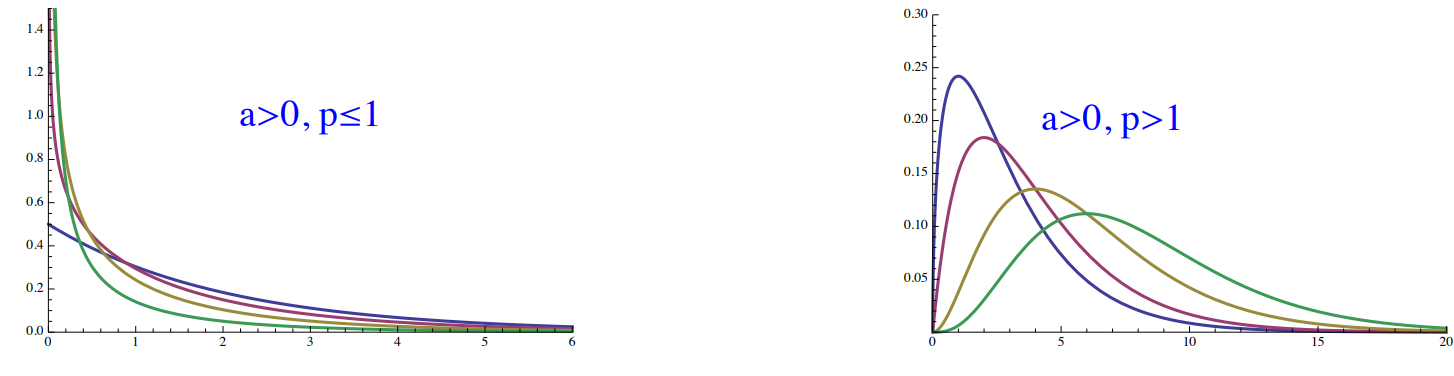
\includegraphics[width=0.8\textwidth]{parametros.png}
\end{align*}

\begin{prop}
Si $X \sim Ga(a,p)$ entonces
\begin{enumerate}
    \item[(1)] Sea $Y = cX$ entonces $Y \sim Ga\left( \frac{a}{c}, p \right)$.
    \item[(2)] Sea $Y = X/a$ entonces $Y \sim Ga(a^2,p)$.
    \item[(3)] Sea $Y = pX$ entonces $Y \sim Ga\left( \frac{a}{p},p\right)$.
    \item[(4)] Sea $Y = X/p$ entonces $Y \sim Ga(ap, p)$.
    \item[(5)] Sea $Y = 1/X$ entonces $Y \sim GaI(a,p)$ con función de densidad dada por
    \begin{align*}
        f_Y(y) = \frac{a^p}{\Gamma(p)}e^{-a\frac{1}{y}}\left(\frac{1}{y}\right)^{p+1}, \ y > 0.
    \end{align*}
    \item[(6)] Las distribución Gamma es reproductiva respecto de p. Sean $X_1,...,X_n$ variables aleatorias independientes tales que $X_i \sim Ga(a, p_i)$, entonces
    \begin{align*}
        S = \sum_{i=1}^{n}{X_i} \sim Ga\left( a, \sum_{i=1}^{p}{p_i} \right).
    \end{align*}
\end{enumerate}
\end{prop}

\subsection{Distribución Chi-Cuadrada}

\begin{defi}
Decimos que $X$ se distribe según una chi cuadrada con n grados de libertad, $X \sim \chi_n^2$, si $X \sim Ga\left( \frac{1}{2}, \frac{n}{2}\right)$ con $n \in \mathbb{N}$. Su función de densidad viene dada por
\begin{align*}
    f(x) = \left\{ \begin{array}{lcc}
             0 &  si  & x \leq 0\\
             \frac{\left( \frac{1}{2}\right)^{n/2}}{\Gamma(n/2)}e^{-x/2}x^{\frac{n}{2} - 1} &  si  & x > 0\\
             \end{array}
        \right. ,
\end{align*}
\end{defi}

\begin{obs}
Si $X \sim \chi_n^2$ entonces
\begin{itemize}
    \item $E[X] = n$.
    \item $V[X] = 2n$.
    \item $M_X(t) = \left( 1 - \frac{1}{2t} \right)^{n/2}$ si $t < \frac{1}{2}$.
\end{itemize}
\end{obs}

\begin{prop}
\begin{enumerate}
    \item[(1)] Si $X \sim U[0,1]$ y si $Y = -2\log(X)$ entonces $Y \sim \chi_2^2$.
    \item[(2)] Si $X \sim N(\mu, \sigma)$ y si $Y = \left( \frac{X - \mu}{\sigma}\right)^2$ entonces $Y \sim \chi_1^2$.
    \item[(3)] Si $X_1,...,X_n$ son variables aleatorias independientes con $X_i \sim N(0,1)$ para todo $i$ entonces $\sum_{i=1}^{n}{X_i^2} \sim \chi_n^2$.
    \item[(4)] Si $X_1,...,X_n$ son variables aleatorias independientes con $X_i \sim \chi_{n_i}^2$ entonces $\sum_{i=1}^{n}{X_i^2} \sim \chi_m^2$ con $m = \sum_{i=1}^{n}{n_i}$.
    \item[(5)] Convergencia en ley a la normal: $\chi_n^2 \xrightarrow[]{ \ \ l \ \ } N(n, \sqrt{2n})$. Además
    \begin{align*}
        Z_n= \sqrt{2\chi_n^2} - \sqrt{2n -1} \xrightarrow[]{ \ \ l \ \ } N(0,1).
    \end{align*}
\end{enumerate}
\end{prop}

\section{Distribución de Erlang}

\begin{defi}
Se dice que una variable aleatoria $X \sim Er(k, \lambda)$ si $X \sim Ga(a = \lambda, p = k)$, $k \in \mathbb{N}$, $\lambda > 0$.
\end{defi}

\begin{obs}
Si $X_1, ..., X_n$ son variables aleatorias independientes tales que $X_i \sim Er(k_i, \lambda)$ entonces
$\sum_{i=1}^{n}{X_n} \sim Er\left( \sum_{i=1}^{n}{k_i}, \lambda\right)$.
\end{obs}

\section{Distribución Beta}

\begin{defi}
Se dice que una variable aleatoria $X \sim Be(\alpha, \beta)$ con $\alpha > 0$, $\beta > 0$ si su función de densidad es
\begin{align*}
    f(x) = \left\{ \begin{array}{lcc}
             \frac{1}{B(\alpha, \beta)}x^{\alpha - 1}(1 - x)^{\beta - 1} &  si  & 0 \leq x \leq 1\\
             0 &  si  & resto\\
             \end{array}
        \right. 
\end{align*}
donde
\begin{align*}
    B(\alpha, \beta) = \int_{0}^{1}{x^{\alpha - 1}(1 - x)^{\beta - 1} \ dx} = \frac{\Gamma(\alpha)\Gamma(\beta)}{\Gamma(\alpha + \beta)}.
\end{align*}
\end{defi}

\begin{obs}
El momento ordinario de orden $k$ respecto del origen
\begin{align*}
    m_k = E[X^k] = \int_{0}^{1}{x^k\frac{\Gamma(\alpha + \beta)}{\Gamma(\alpha)\Gamma(\beta)}x^kx^{\alpha -1}(1-x)^{\beta -1} \ dx} = \frac{\Gamma(\alpha + \beta)}{\Gamma(a)} \cdot \frac{\Gamma(\alpha + k)}{\Gamma(\alpha + \beta + k)}.
\end{align*}
En particular
\begin{itemize}
    \item $m_1 = \frac{\alpha}{\alpha + \beta}$.
    \item $m_2 = \frac{(\alpha + 1)\alpha}{(\alpha + \beta)(\alpha + \beta + 1)}$.
\end{itemize}
\end{obs}

\section{Aproximación de distribuciones}

\begin{defi}
Sea $\{X_n\}$ una sucesión de variables aleatorias definidas todas ellas sobre un mismo espacio de probabilidad. Diremos que la sucesión converge en ley o distribución hacia la variable aleatoria X, definida en el mismo espacio de probabilidad, si y solo si la correspondiente sucesión de funciones de distribución $\{F_n\}$ converge hacia la función de distribución F de la variable aleatoria X en todo punto de continuidad de F.
\end{defi}

\subsection{Teoremas de caracterización de la convergencia en ley para variables aleatorias discretas}

\begin{teo}
Si la sucesión de variables aleatorias $\{X_n\}$ toma valores enteros no negativos, para todo n, entonces la condición necesaria y suficiente para que dicha sucesión converja en ley hacia una variable aleatoria discreta X es
\begin{align*}
    \lim_{n \to \infty}{P(X_n = k) = P(X = k)} \ \ \ para \ todo \ k \in \mathbb{N}.
\end{align*}
\end{teo}

\begin{teo}
Si existe la función generatriz de probabilidad $G_n(s)$ para cada una de las variables aleatorias $X_n$ y existe la función generatriz de probabilidad de la variable aleatoria X, $G_X(s)$, de la variable aleatoria límite, entonces
\begin{align*}
    \lim_{n \to \infty}{G_n(s) = G_X(s)} \ \ \ \text{para todo s donde } G_X(s) \ exista.
\end{align*}
En este caso la sucesión $\{X_n\}$ converge en ley o distribución hacia la variable aleatoria X.
\end{teo}

\subsection{Aproximación de una distribución Binomial por una distribución de Poisson}

La distribución de Poisson surgió como una convergencia de la distribución Binomial de parámetros $n$ y $p$ con las siguientes condiciones
\begin{itemize}
    \item $n \to +\infty$.
    \item $p \to 0$.
    \item $np \to \lambda$, con $\lambda$ constante.
\end{itemize}
En tales condiciones la distribución Binomial se puede aproximar por una distribuión de Poisson de parámetro $\lambda = np$ (Teorema de Poisson).
\\
\newline
Obsérvese que la media de la distribución $Bi(n,p)$ es $np$ que coincide con la media de la distribución $Po(\lambda = np)$. Sin embargo, la varianza de la distribución $Bi(n,p)$ es $nqp$ y la de la distribución $Po(\lambda = np)$ es $np$. Por lo tanto esta aproximación será más exacta cuanto más próximo a 1 sea $q$ y por lo tanto cuanto más próximo a cero sea $p$.

\subsection{Teoremas de caracterización de la convergencia en ley para variables aleatorias absolutamente continuas}

\begin{teo}
Sean $\{X_n\}$ y X variables aleatorias absolutamente continuas con funciones de densidad $f_n$ y $f$ respectivamente, tales que 
\begin{align*}
    \lim_{n \to \infty}{f_n(x) = f(x)} \ \ \text{para casi todo x}.
\end{align*}
Entonces la sucesión de variables aleatorias converge en ley hacia la variable aleatoria X.
\end{teo}

\begin{teo}
Sean $\{X_n\}$ y X variables aleatorias absolutamente continuas con funciones de densidad $f_n$ y $f$ respectivamente, y funciones generatrices de momentos $M_n(t)$ y $M(t)$ respectivamente, tales que
\begin{align*}
    \lim_{n \to \infty}{M_n(t) = M(t)},
\end{align*}
para todos los valores de t en un intervalo alrededor del punto 0. Entonces la sucesión de variables aleatorias converge en ley hacia la variable aleatoria X.
\end{teo}

\begin{obs}
\begin{itemize}
    \item Este último teorema es válido tanto para variables discretas como para variables continuas.
    \item No solo es posible aproximar distribuciones discretas por discretas, también es posible la aproximación de una distribución discreta por una distribución continua. En la mayoría de los casos se suele hacer mediante una distribución normal.
\end{itemize}
\end{obs}

\subsection{Teorema central del límite}

\begin{defi}
Sea $\{X_n\}$ una sucesión de variables aleatorias, definidas todas ellas sobre el mismo espacio de probabilidad, con medias y varianzas finitas. Diremos que la sucesión $\{X_n\}$ obedece al teorema central del límite si y solo si $\{Z_n\}$ converge en ley a una distribución $N(0,1)$, siendo
\begin{align*}
    Z = \frac{S_n - E[S_n]}{\sigma(S_n)}
\end{align*}
con $S_n = \sum_{i=1}^{n}{X_i}$.
\end{defi}

\begin{teo}[Teorema de Moivre]
Sea $\{X_n\}$ una sucesión de variables aleatorias independientes e idénticamente distribuidas, cada una de ellas $Bi(n = 1, p)$ (o lo que es lo mismo $Ber(p)$). Entonces la sucesión obedece al teorema central del límite.
\end{teo}

\begin{cor}
Si $X \sim Bi(n,p)$ y $n$ es grande, la distribución de X se puede aproximar mediante $N(np, \sqrt{npq})$.
\end{cor}

